\documentclass[../main.tex]{subfiles}
\begin{document}
\section{大模型架构基础}\label{sec:llm-architecture}
\subsection{自然语言处理任务基础}
\begin{enumerate}
    \item \textbf{分词}\footnote{就是把自然语言构建出一个词汇表，不能切分太细使得词表太大，也不能切分太粗丧失语义自由度。之后用Tokenizer这个结构可以将文本转换为独立的 token 序列，再进一步变成模型可处理的向量形式}
    \begin{enumerate}
        \item \textbf{Token：}令牌\footnote{现译作“词元”}，通过分词技术将一句话分割成的最小单位，是一个特定 NLP 模型能处理的最基本元素。
        
        \item \textbf{分词作用：}分词需要在词汇表大小和序列长度之间取得平衡，也是模型输入构造的关键一步。

        \item \textbf{传统分词方法的挑战：}
        \begin{itemize}
            \item \textbf{全词切分\footnote{直接把一个单词作为一个token}的问题：}
            {\small\kaishu
            \begin{itemize}
                \item 词汇表过大：词汇量会随语料库不断增长，模型训练和部署困难；
                \item OOV（Out-Of-Vocabulary）问题：未在训练数据中出现的新词、复合词、人名、拼写错误等都会被标记为 \texttt{<UNK>}。
            \end{itemize}
            }
            \item \textbf{字符切分\footnote{直接把一个字母作为一个token}的问题：}
            {\small\kaishu
            \begin{itemize}
                \item 词汇表较小，基本没有 OOV 问题；
                \item 但序列过长，计算量大，且难以捕捉长距离语义依赖。
            \end{itemize}
            }
        \end{itemize}

        \item \textbf{Subword 分词：}将一个词分解成更小的、具有语义或统计意义的片段（subwords），以在全词切分和字符切分之间取得平衡，确保：
        {\small\kaishu
        \begin{itemize}
            \item 词汇表规模适中：高频词可整体保留，又避免词表无限膨胀；
            \item OOV 问题得到缓解：任意未见词都可拆成已知子词序列；
            \item 语义可解释性较强：子词通常比单字符更有意义（如 \texttt{un}、\texttt{ing} 等）。
        \end{itemize}
        }
        
        \begin{enumerate}
            \item \textbf{BPE（Byte Pair Encoding）：}
            \begin{itemize}
                \item 从字符级词表开始；
                \item 将单词先拆成单字符，并加入特殊词尾标记（如 \texttt{</w>}）以保留词边界；
                \item 统计语料中频率最高的相邻字符对；
                \item 将最高频字符对合并为新的子词单元；
                \item 重复该过程，直到词汇表达到目标规模。
            \end{itemize}

            \item \textbf{WordPiece：}
            \begin{itemize}
                \item 与 BPE 的区别在于：BPE 按\textbf{最高频率}合并，WordPiece 按\textbf{似然提升最大}进行合并\footnote{换句话说，BPE是直接看出现的绝对频率，而wordpiece要确保两个token合并后出现的概率，比单独的出现其中任意一个要高，这样合并才有价值}；
                \item 常用打分可写为：
                $$
                \text{score}=\log p(ab)-(\log p(a)+\log p(b))
                =\log \frac{p(ab)}{p(a)p(b)}
                $$
                \item 基本步骤：先构建 char 级词表，再不断合并能最大提升句子似然的片段，直到达到预定词表大小或收益低于阈值。
            \end{itemize}

            \item \textbf{SentencePiece：}
            \begin{itemize}
                \item 直接把整个句子视为整体进行编码，而不依赖预分词；
                \item 内置 BPE、Unigram、char 和 word 等多种分词方法；
                \item 通常直接基于 Unicode 编码整个句子，空格也会被特殊编码；
                \item 相比传统实现进行了工程优化，分词速度更快。
            \end{itemize}
        \end{enumerate}
    \end{enumerate}

    \item \textbf{词向量和词嵌入}
    \begin{itemize}
        \item \textbf{词向量：}词的特征分布表示\footnote{分词分好的词表中，每一个token都固定对应一个数值的向量}，是 NLP 模型层与层之间传递信息的数据形式；
        \item \textbf{词嵌入：}本质上与词向量指向同一对象，只是更强调它在神经网络中的数据存在形式\footnote{这个解释很诡异吗，应该是词嵌入是一个过程，词向量是该过程生成的结果}；
        \item 若词表大小为 $n$，每个 token 的特征维度为 $m$，则词向量矩阵可表示为\footnote{就是说每一个词嵌入后变成一个m维的向量}
        $$
        \begin{bmatrix}
        V_1\\
        \vdots\\
        V_n
        \end{bmatrix}
        =
        \begin{bmatrix}
        V_{11} & \cdots & V_{1m}\\
        \vdots & \ddots & \vdots\\
        V_{n1} & \cdots & V_{nm}
        \end{bmatrix}
        $$
        \item 学习后的词向量通常能把语义相近的词映射到向量空间中相近的位置。
    \end{itemize}

    \item \textbf{句子的 one-hot 编码表示}
    \begin{itemize}
        \item \textbf{方式一：二维稀疏矩阵。}将句中每个 token 分别表示为一个 one-hot 向量，再按顺序堆叠成矩阵（就是上面那个）；
        \item \textbf{方式二：一维稠密索引序列。}直接将每个 token 映射为词表中的编号（比如“我”对应id 10086，“恨”对应id 114514，“人机”对应id 666，那么这句话就写成$[10086,114514,666]$）
    \end{itemize}

    \item \textbf{文本相似度}
    \begin{itemize}
        \item 常见相似度或距离度量包括：
        \begin{itemize}
            \item \textbf{余弦相似度：}
            $$
            \cos \theta = \frac{A\cdot B}{\lVert A\rVert \lVert B\rVert}
            $$
            值越大，文本越相似；
            
            \item \textbf{欧式距离：}
            $$
            d=\sqrt{\sum_{i=1}^{n}(x_i-y_i)^2}
            $$
            距离越小，文本越相似；
            
            \item \textbf{曼哈顿距离：}
            $$
            d=\sum_{i=1}^{n}|x_i-y_i|
            $$
            距离越小，文本越相似；
            
            \item \textbf{Jaccard 相似度：}
            $$
            J(A,B)=\frac{|A\cap B|}{|A\cup B|}
            $$
            或向量形式
            $$
            \mathrm{EJ}(A,B)=\frac{A\cdot B}{\lVert A\rVert^2+\lVert B\rVert^2-A\cdot B}
            $$
            值越大，文本越相似。
        \end{itemize}
    \end{itemize}
\end{enumerate}
\subsection{传统NLP模型}
\begin{enumerate}
    \item \textbf{词袋模型：}
    \begin{itemize}
        \item \textbf{原理：}将文本表示为一个词的集合，忽略词语的上下文关系，只统计词语出现的频率等信息；
        \item \textbf{问题：}不考虑词序和上下文，例如 GAI 与 AGI 会被视为相同。
    \end{itemize}

    \item \textbf{朴素贝叶斯分类器：}
    \begin{itemize}
        \item \textbf{定义：}在条件独立假设下，对样本进行分类：
        $$
        v_{NB}=\arg\max_{v_j\in V} P(v_j)\prod_i P(a_i\mid v_j)
        $$
        \item \textbf{思想：}与直接估计
        $$
        P(a_1,\ldots,a_n\mid v_j)
        $$
        相比，估计各项
        $$
        P(a_i\mid v_j)
        $$
        所需数据量小得多；
        \item \textbf{特点：}若条件独立性成立，则朴素贝叶斯分类等价于 MAP 分类；否则只是近似；
        \item \textbf{优缺点：}在单词数量大且方差较小时，计数估计效果较好；但当特征较少时，Logistic 回归、神经网络或 SVM 往往更优。
    \end{itemize}

    \item \textbf{N元单词模型（N-gram）：}
    \begin{itemize}
        \item \textbf{核心假设（马尔可夫假设）：}一个词的出现只依赖于它前面的 $N-1$ 个词，而与更早的词无关：
        $$
        P(w_i\mid w_1,\ldots,w_{i-1})\approx P(w_i\mid w_{i-(N-1)},\ldots,w_{i-1})
        $$
        \item \textbf{定义：}用于计算句子或词语序列的概率：
        $$
        P(S)=P(w_1,\ldots,w_m)\approx \prod_{i=1}^{m} P(w_i\mid w_{i-(N-1)},\ldots,w_{i-1})
        $$
        \item \textbf{常见类型：}
        \begin{itemize}
            \item \textbf{1-gram（Unigram）：}不依赖任何前文；
            \item \textbf{2-gram（Bigram）：}只依赖前一个词；
            \item \textbf{3-gram（Trigram）：}依赖前两个词。
        \end{itemize}
        \item \textbf{参数估计：}通常采用最大似然估计（MLE）：
        $$
        P(w_i\mid w_{i-(N-1)},\ldots,w_{i-1})
        =\frac{\mathrm{Count}(w_{i-(N-1)},\ldots,w_i)}
        {\mathrm{Count}(w_{i-(N-1)},\ldots,w_{i-1})}
        $$
        {\small\kaishu
        例如，在二元模型（Bigram）中，
        $$
        P(\text{饭}\mid \text{吃})
        =
        \frac{\mathrm{Count}(\text{吃,饭})}{\mathrm{Count}(\text{吃})}
        $$
        若训练语料为：
        \[
        \text{我吃饭，\quad 你吃饭，\quad 我吃面，\quad 我不吃饭}
        \]
        则：
        \[
        \mathrm{Count}(\text{吃})=4,\qquad \mathrm{Count}(\text{吃,饭})=3
        \]
        因此：
        $$
        P(\text{饭}\mid \text{吃})=\frac{3}{4}
        $$
        这表示：在所有前一个词是“吃”的情况中，下一个词是“饭”的比例为 $\frac{3}{4}$。
        }
        \item \textbf{问题：}当 $N$ 增大时，许多合理的 N-gram 在训练语料中未出现，导致 $\mathrm{Count}=0$；
        \item \textbf{后果：}MLE 给出的某些条件概率为 $0$，进而整个句子概率也可能为 $0$；
        \item \textbf{取舍：}$N$ 越大，模型越准确但数据稀疏性越严重；$N$ 越小，泛化更好但上下文信息不足。
        \item \textbf{平滑技术：}将部分概率质量从高频 N-gram 分配给低频或未出现的 N-gram，避免概率为零。
        \begin{itemize}
            \item \textbf{加一平滑：}给每个统计单元的计数都加 $1$，例如
            $$
            P_{\mathrm{Add1}}(w_i\mid w_{i-1})
            =\frac{C(w_i,w_{i-1})+1}{C(w_{i-1})+|V|}
            $$
            \item \textbf{回退平滑：}当高阶 N-gram 计数不足时，退回到低阶模型（如 $N-1,N-2,\ldots$）。
        \end{itemize}
        \item \textbf{评价：}N 元模型实现简单、速度快，曾广泛应用于语音识别、早期机器翻译和拼写纠错，但其局限在于难以建模长距离依赖，且严重依赖计数。
    \end{itemize}

    \item \textbf{Word2Vec：}
    \begin{itemize}
        \item \textbf{定义：}能够将词语映射到低维稠密向量空间，从而捕获语义关系；
        \item \textbf{对比 One-Hot：}
        \begin{itemize}
            \item One-Hot 用高维稀疏向量表示词，优点是简单且唯一；
            \item 缺点是维度高、稀疏，且无法表达词语之间的语义相似性。
        \end{itemize}
        \item \textbf{分布式语义表示：}基于“一个词的含义由其上下文决定”的思想，将词语映射到低维、稠密、可表示语义相似度的实数向量空间；
        \item \textbf{作用：}通过训练获得低维稠密词向量，避免 One-Hot 的维度灾难，并能通过向量距离衡量语义关系。
    \end{itemize}

    \item \textbf{Seq2Seq：}
    \begin{itemize}
        \item \textbf{背景：}自然语言具有高度非结构化和动态长度特性；
        \item \textbf{传统模型限制：}传统全连接网络或 CNN 往往要求固定输入和输出维度，难以处理变长输入输出问题；
        \item \textbf{典型场景：}
        \begin{itemize}
            \item 机器翻译中，源语言句子和目标语言句子长度通常不相等；
            \item 自动问答中，输入可能很短，而输出答案可能较长。
        \end{itemize}
        \item \textbf{核心思想：}使用编码器网络将输入序列编码为固定维度向量或一系列隐状态，再由解码器网络逐步生成目标序列；
        \item \textbf{意义：}首次提供了统一的变长输入到变长输出的深度学习框架，突破了固定长度处理的限制。
    \end{itemize}
\end{enumerate}
\subsection{Transformer结构与自注意力机制}\label{sec:transformer-self-attention}
\begin{enumerate}
    \item \textbf{前Transformer时代}
    \begin{itemize}
        \item \textbf{RNN（循环神经网络）}
        \begin{figure}[H]
            \centering
            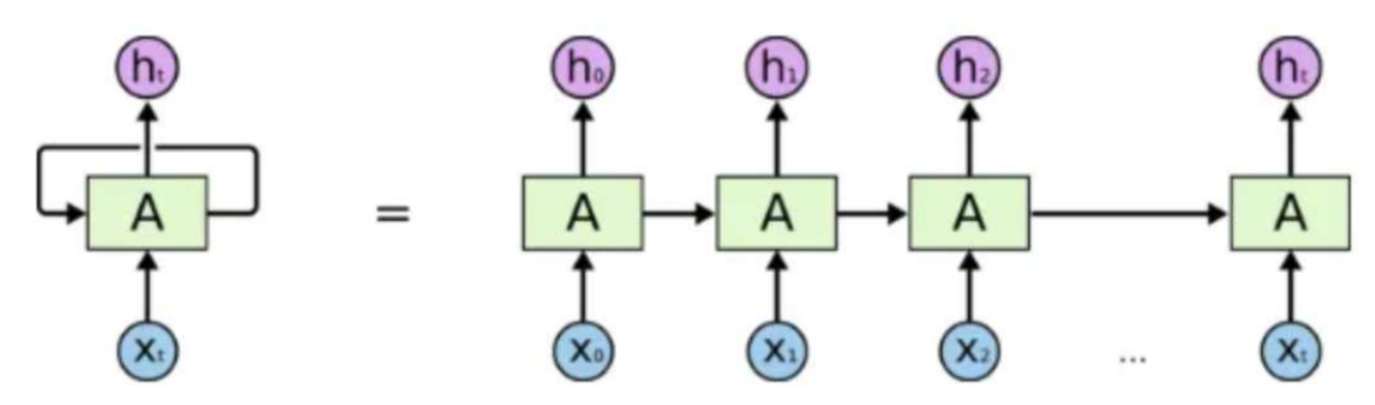
\includegraphics[width=0.5\linewidth]{images/RNN.png}
            \caption{RNN结构示例}
            \label{fig:placeholder}
        \end{figure}
        \begin{itemize}
            \item \textbf{原理：}通过隐藏状态(Hidden State)将前一个时间步的信息传递给下一个时间步，从而具备了“记忆”能力，能够理解文本、语音等序列的上下文依赖关系。
            \item \textbf{核心局限性}
            \begin{enumerate}
                \item 长距离依赖捕获困难：信息在多轮传递中丢失
                \item 训练速度慢：训练过程必须按顺序进行，无法利用GPU并行计算能力
                \item 梯度消失或梯度爆炸
                \item 词汇表限制，OOV问题
            \end{enumerate}
        \end{itemize}
        \item \textbf{LSTM}
        \begin{itemize}
        \begin{figure}[H]
            \centering
            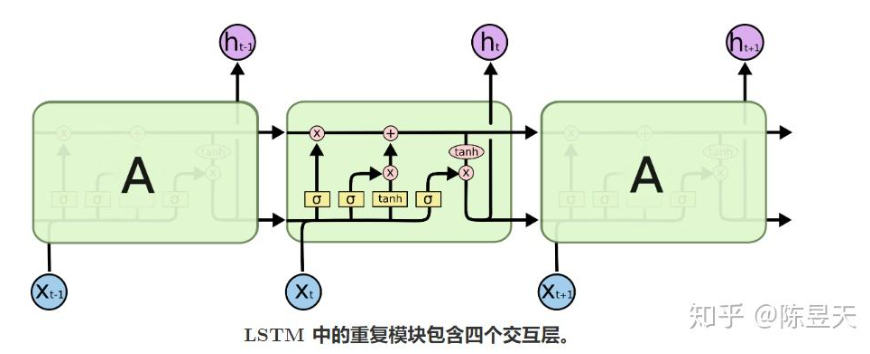
\includegraphics[width=0.5\linewidth]{images/LSTM.png}
            \caption{LSTM结构示例}
            \label{fig:placeholder}
        \end{figure}
            \item \textbf{原理：}通过三个关键门控机制(遗忘门、输入门、输出门)和细胞状态(Cell State)
            \item \textbf{对RNN局限性克服：}
            \begin{enumerate}
                \item \textbf{解决梯度消失：}细胞状态线性传递，梯度有效反向传播；
                \item \textbf{增强长期记忆：}门控机制可以记忆和遗忘
                \item \textbf{更高的性能}
            \end{enumerate}            
            \item \textbf{核心局限性}
            \begin{enumerate}
                \item 信息瓶颈：细胞状态和隐藏状态都必须将整个长序列上下文压缩
                \item 训练速度慢：训练过程必须按顺序进行，无法利用GPU并行计算能力
                \item 计算复杂度高：比Transformer还高
            \end{enumerate}
        \end{itemize}
    \end{itemize}
    \item \textbf{Transformer具体原理：}参考\href{https://www.bilibili.com/video/BV13z421U7cs/?spm_id_from=333.337.search-card.all.click&vd_source=5deca47094767260f853b759a625a68f}{B站视频}
    \item \textbf{Transformer模型家族：}
    \begin{itemize}
        \item 纯Encoder模型（自编码模型）：句子分类、实体识别等需要全面上下文任务，例如Bert
        \item 纯Decoder模型（自回归模型）：掩码自注意力机制，文本生成任务，例如GPT
        \item Encoder-Decoder模型（Seq2Seq）：双向注意力理解，翻译、摘要和生成式问答，例如T5
    \end{itemize}
  
\end{enumerate}
\subsection{预训练-微调范式及其演进}
\begin{enumerate}
    \item \textbf{预训练}
    \begin{itemize}
        \item Transformer模型本质上都是预训练语言模型，采用自监督学习方式在大量语料上训练
        \begin{itemize}
            \item 因果语言建模（用前N个词预测下一个词）
            \item 遮盖语言建模（用周围词语预测被遮掉的词语）
        \end{itemize}
    \end{itemize}
    \item \textbf{迁移学习（微调）}
    \begin{itemize}
        \item \textbf{优点：}
        \begin{itemize}
            \item 知识继承:激活预训练模型中沉淀的通用统计理解能力。
            \item 数据高效:仅需少量特定任务的标注语料即可达到高性能。
            \item 降本增效:极大地减少了训练所需的计算资源与时间周期。
        \end{itemize}
        \item \textbf{应用场景：}上下文学习（Few Shot）无法解决问题时
        \item \textbf{分类：}
        \begin{enumerate}
            \item \textbf{全微调（Full Fine-Tuning）：}基础模型的所有参数都参与微调，适用于有全新的、足够大的数据，需要对原生模型知识进行较大重构的场景；
            
            \item \textbf{部分微调（Partial Fine-Tuning）：}
            \begin{itemize}
                \item 又称\textbf{高效参数微调}（Parameter-Efficient Fine-Tuning, PEFT）；
                \item 冻结基础模型部分层参数，仅调整未冻结参数；
                \item 是目前最常用的微调方式，通过只训练少量参数达到接近全量微调的效果；
                \item 常见方法包括：LoRA、Adapter Tuning、Prefix Tuning、Prompt Tuning。
            \end{itemize}
            
            \item \textbf{提示词微调（Prompt Tuning）：}通过设计提示词模板及对应输出来适配任务，不更新基础模型参数，仅更新 prompt 对应的 embedding 参数；
            \begin{itemize}
                \item 解决问题：目标差异、头部过拟合
            \end{itemize}
            
            \item \textbf{RLHF（Reinforcement Learning from Human Feedback）：}利用强化学习直接优化带有人类反馈的语言模型，使模型输出更符合人类偏好与价值观。
        \end{enumerate}
        \begin{table}[H]
            \centering
            \caption{全量参数微调与参数高效微调对比}
            \begin{tabular}{p{2.2cm}p{4.6cm}p{4.3cm}p{4.3cm}}
                \toprule
                微调方法 & 原理 & 优点 & 缺点 \\
                \midrule
                全参数微调 & 对预训练模型的所有参数进行微调，以适应特定任务。 & 能够充分利用模型的表达能力，达到较好的性能；不受限于增量矩阵的秩特性，适用于各种任务和数据集。 & 需要大量计算资源，训练时间较长，不利于快速迭代和优化。 \\
                
                PEFT & 通过仅调整少量额外参数来适应新任务，保持大部分预训练模型参数不变。 & 减少了微调参数的数量，降低了训练时间和成本，适用于计算资源有限的情况。 & 可能无法完全发挥模型潜力，性能可能略逊于全参数微调。 \\
                
                LoRA & 基于低秩矩阵分解思想，将原始高维权重矩阵分解为两个低秩矩阵的乘积，以减少可训练参数量和计算复杂度。 & 降低了存储需求和计算成本，提高了训练速度与推理速度。 & 可能降低模型准确性；适用性受限，主要适用于具有低秩特性的增量矩阵。 \\
                \bottomrule
            \end{tabular}
        \end{table}
        \item \textbf{LoRA（Low-Rank Adaptation of LLM）：}
        \begin{itemize}
            \item \textbf{核心思想：}将参数更新量写成低秩分解形式，用极少的可训练参数近似完整参数更新；
            \item 设原始预训练权重为 $W_0$，微调后权重为
            $$
            W_0+\Delta W
            $$
            在 LoRA 中，冻结 $W_0$，只训练两个低秩矩阵 $A,B$，使
            $$
            W_0+\Delta W = W_0+BA
            $$
            其中
            $$
            B\in \mathbb{R}^{d\times r},\qquad A\in \mathbb{R}^{r\times k}
            $$
            \item 当秩 $r$ 很小时，可训练参数量远小于原始权重矩阵，从而显著降低微调成本。
        \end{itemize}
        
        \item \textbf{RLHF（Reinforcement Learning from Human Feedback）：}
        \begin{itemize}
            \item \textbf{核心思想：}将人类反馈纳入奖励函数，利用强化学习优化语言模型，使其输出更符合人类目标、偏好和需求；
        \end{itemize}
    \end{itemize}
\end{enumerate}

\end{document}
